\documentclass[11pt]{report}
\usepackage[spanish]{babel}
\usepackage[utf8]{inputenc}
\usepackage{amsmath}
\usepackage{amssymb}
\usepackage{graphicx}
\graphicspath{ {images/} }

\begin{document}{}
\title{Matemáticas para las Ciencias Aplicadas III \\ Tarea 2}
\maketitle

\textbf{Anton-Bivens-Davis} \\

\textbf{Sección 14.2} \\

\textbf{15-18} Evaluate the double integral in two ways using iterated integrals:
(a) viewing $R$ as a type I region, and (b) viewing $R$ as a type II region.

\textbf{18.} \\

$ {\displaystyle \iint \limits_R } \, y \, \, \text dA; \, R$ is the region in the first
quadrant enclosed between the circle $x^2 + y^2 = 25$ and the line $x + y = 5$. \\

\textbf{19-24.} Evaluate the double integral in two ways using iterated integrals: \\

\textbf{22.} $ {\displaystyle \iint \limits_R } \, x \, \, \text dA; \, R$ is the region
enclosed by $y = sin^{-1} x, x = \frac{1}{\sqrt{2}},$ and $y = 0$. \\

\textbf{28.} \\

(a) By hand or with the help of a graphing utility, make a sketch of the region
$R$ enclosed between the curves $y = 4x^3 - x^4$ and $y = 3 - 4x + 4x^2$. \\

(b) Find the intersections of the curves in part (a). \\

(c) Find $ {\displaystyle \iint \limits_R } \, x \, \, \text dA $ \\

\textbf{37-38} Use double integration to find the volume of the solid. \\

\textbf{37.} \\

\begin{figure}[h]
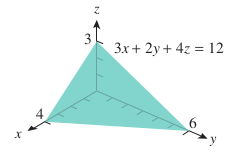
\includegraphics[scale=0.5]{img1.png}
\centering
\end{figure}

\textbf{57.} Try to evaluate the integral with a CAS using the stated order of
integration, and then by reversing the order of integration.\\

(a) $ {\displaystyle \int \limits_0^4 \int \limits_{\sqrt{x}}^2 } \, \sin{\pi y^3} \, \, \text dx \text dy $ \\

(b) $ {\displaystyle \int \limits_0^1 \int \limits_{sin^{-1}y}^{\frac{\pi}{2}} } \, \sec{\cos{x}}^2 \, \, \text dx \text dy $ \\

\textbf{59.} Evaluate $ {\displaystyle \iint \limits_R } \, xy^2 \, \, \text dA $ over
the region R shown in the accompanying figure. \\
\begin{figure}[h]
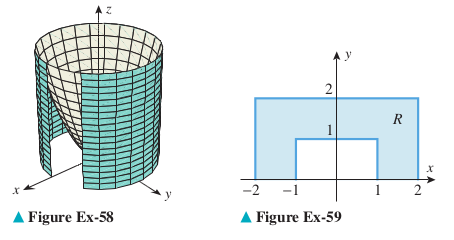
\includegraphics[scale=0.5]{img2.png}
\centering
\end{figure}

\textbf{63.} Suppose that the temperature in degrees Celsius at a point $(x, y)$
on a flat metal plate is $T(x, y) = 5xy + x^2 $, where $x$ and $y$ are in meters.
Find the average temperature of the diamond-shaped portion of the plate for which
$|2x + y| \leq 4$ and $|2x - y| \leq 4$. \\

\textbf{Sección 14.5} \\

\textbf{12.} $ {\displaystyle \iiint \limits_G } \, \cos{\frac{z}{y}} \, \, \text dV $,
where $G$ is the solid defined by the inequalities
$\frac{\pi}{6} \leq y \leq \frac{\pi}{2}, y \leq x \leq \frac{\pi}{2}, 0 \leq z \leq xy$. \\


\textbf{37.} Let $G$ be the tetrahedron in the first octant bounded by the
coordinate planes and the plane \\

\[ \frac{x}{a} + \frac{y}{b} + \frac{z}{c} = 1, (a > 0, b > 0, c > 0) \]

(a) List six different iterated integrals that represent the volume of $G$. \\

(b) Evaluate any one of the six to show that the volume of $G$ is $\frac{1}{6} abc$. \\

\textbf{38.} Use a triple integral to derive the formula for the volume of the ellipsoid

\[ \frac{x^2}{a^2} + \frac{y^2}{b^2} + \frac{z^2}{c^2} = 1 \]

\textbf{Hughes-Hallet} \\

\textbf{Sección 16.2}

\textbf{35.} \\

\[ \int \limits_0^1 \, \int \limits_{\sqrt{y}}^1 \sqrt{2 + x^3} \, \text dx \, \text dy \]

\textbf{37.} \\

\[ \int \limits_0^1 \, \int \limits_{e^y}^e \frac{x}{\ln{x}} \, \text dx \, \text dy \]

\textbf{60.} Show that for a right triangle the average distance from any point
in the triangle to one of the legs is one-third the length of the other leg.
(The legs of a right triangle are the two sides that are not the hypotenuse.) \\

\textbf{62.} Find the area of the crescent-moon shape with circular arcs as edges
and the dimensions shown in Figure 16.22. \\

\textbf{Sección 16.3} \\

In Problems 14–18, decide whether the integrals are positive,negative, or zero.
Let $S$ be the solid sphere $x^2 + y^2 + z^2 \leq 1$, and $T$ be the top half of
this sphere (with $z \geq 0$), and $B$ be the bottom half (with $z \leq 0$), and $R$
be the right half of the sphere (with $x \geq 0$), and $L$ be the left half
(with $x \leq 0$). \\

\textbf{14.} \\

\[ \int _T e^z \, \text dV \]

\textbf{15.} \\

\[ \int _B e^z \, \text dV \]

\textbf{16.} \\

\[ \int _S \sin{z} \, \text dV \]

\textbf{17.} \\

\[ \int _T \sin{z} \, \text dV \]

\textbf{18.} \\

\[ \int _R \sin{z} \, \text dV \]

\textbf{31.} A trough with triangular cross-section lies along the $x$-axis for
$0 \leq x \leq 10$. The slanted sides are given by $z = y$ and $z = -y$ for
$0 \leq z \leq 1$ and the ends by $x = 0$ and $x = 10$, where $x, y, z$ are in meters.
The trough contains a sludge whose density at the point $(x, y, z)$ is
$\delta = e^{-3x}$ kg per $m^3$. \\

\textbf{a)} Express the total mass of sludge in the trough in terms of triple
integrals. \\

\textbf{b)} Express the total mass of sludge in the trough in terms of triple
integrals. \\

\textbf{55.} $E$ is the region bounded by $x = 0, y = 0, z = 0, z = 2,$
and $2x + 4y + z = 4$. \\

\textbf{57.} Figure 16.28 shows part of a spherical ball of radius 5 cm.
Write an iterated triple integral which represents the volume of this region. \\

\textbf{66.} Find the center of mass of the tetrahedron that is bounded by the
$xy, yz, xz$ planes and the plane $x + 2y + 3z = 1$. Assume the density is
1 $gm/cm^3$ and $x, y, z$ are in centimeters. \\

Problems 67–69 concern a rotating solid body and its \textit{moment of inertia}
about an axis; this moment relates angular acceleration to torque (an analogue
of force). For a body of constant density and mass $m$ occupying a region $W$
of volume $V$ , the moments of inertia about the coordinate axes are

\[I_x = \frac{m}{V} \int _W (y^2 + z^2) \, \text d V \]

\[I_y = \frac{m}{V} \int _W (x^2 + z^2) \, \text d V \]

\[I_z = \frac{m}{V} \int _W (x^2 + z^2) \, \text d V \]

\textbf{67.} Find the moment of inertia about the $z$-axis of the rectangular
solid of mass $m$ given by $0 \leq x \leq 1, 0 \leq y \leq 2, 0 \leq z \leq 3$. \\

Are the statements in Problems 74–83 true or false? Give reasons for your answer. \\

\textbf{75.} The region of integration of the triple iterated integral
$\int_0^1 \int_0^1 \int_0^x f dz dy dx $ lies above a square in the $xy$-plane
and below a plane. \\

\textbf{78.} The iterated integrals $\int_{-1}^1 \int_0^1 \int_0^{1-x^2} f dz dy dx $
and $\int_0^1 \int_0^1 \int_{-\sqrt{1-z}}^{\sqrt{1-z}} f dz dy dx $ are equal. \\


\textbf{80.} If $W$ is the unit cube $0 \leq x \leq 1, 0 \leq y \leq 1, 0 \leq z \leq 1$
and $ \int _W f \, \text dV = 0$, then $f = 0$ everywhere in the unit. \\

\end{document}
